The Run~2 search for heavy resonances in four-top-quark final states has established competitive constraints on a variety of top-philic new physics scenarios. 
However, the analysis is still limited by both statistical uncertainties at high mass and modelling uncertainties in regions with large jet multiplicities. 
The HL-LHC, expected to deliver an integrated luminosity of up to 3~ab$^{-1}$ per experiment at $\sqrt{s}=14$~TeV, will significantly enhance the sensitivity to rare processes such as $pp \to t\bar{t}t\bar{t}$ and to potential heavy resonances decaying into $t\bar{t}$ pairs.

The large centre-of-mass energy required to produce four top quarks makes this final state particularly sensitive to new particles at the TeV scale. 
In many top-philic models, the production cross-section decreases rapidly with increasing resonance mass, such that the achievable sensitivity critically depends on both the available integrated luminosity and the control of systematic uncertainties. 
It is therefore essential to evaluate how the search reach evolves under HL-LHC conditions and to identify whether future improvements will be dominated by increased statistics or by improved theoretical and experimental modelling.

In the following, the sensitivity of the heavy-resonance searches is extrapolated to HL-LHC conditions, based on the Run~2 analysis strategy and under different assumptions on the evolution of systematic uncertainties.

\subsection{Extrapolation Framework}
\label{sec:HL_framework}

The extrapolation to HL-LHC conditions is performed by scaling the Run~2 analysis to proton--proton collisions at $\sqrt{s}=14$~TeV and to an integrated luminosity of up to 3~ab$^{-1}$ per experiment. 
All signal and background cross-sections are rescaled to their corresponding values at 14~TeV, while statistical uncertainties are scaled according to the assumed integrated luminosity.

Two scenarios are considered to evaluate the impact of systematic uncertainties on the projected sensitivity. 
In the first scenario (S1), all systematic uncertainties are retained at their Run~2 values, providing a conservative estimate of the achievable performance at the HL-LHC. 
Several nuisance parameters that were constrained in the Run~2 profile likelihood fit, such as the normalisation of $t\bar{t}W$ production and non-prompt lepton backgrounds, are fixed to their post-fit values in the extrapolation. 
Their associated uncertainties are scaled with the integrated luminosity to reflect the increased statistical precision.

In the second scenario (S2), improvements in theoretical modelling and detector performance are assumed. 
The generator uncertainty for the $t\bar{t}t\bar{t}$ signal is removed due to its significant overlap with other modelling uncertainties, and the remaining signal modelling uncertainties are reduced by approximately a factor of two compared to Run~2. 
For background processes, in particular $t\bar{t}W$ production which constitutes the dominant background in the multilepton channel, modelling uncertainties are also reduced. 
Uncertainties associated with data-driven background estimates that are statistically limited are scaled with luminosity, while discrepancies observed between data and simulation are conservatively retained.

Experimental uncertainties are assumed to scale with the integrated luminosity, reflecting the improved calibration precision expected with larger datasets.

The detailed treatment of systematic uncertainties in Scenario~2 is summarised in Tables~\ref{tab:HL_syst_2LSS} and~\ref{tab:HL_syst_1L}. 
The projected sensitivities presented below use the same multivariate discriminants and signal-region definitions as in the Run~2 analysis.

\begin{table}[htbp]
\centering
\caption{Systematic uncertainty treatment in Scenario~2 (S2) for the extrapolation of the SM $\boldsymbol{t\bar{t}t\bar{t}}$ measurement and the resonance search in the 2LSS/ML channel.}
\label{tab:HL_syst_2LSS}

\begin{tabular}{p{0.5\textwidth} p{0.3\textwidth}}
\toprule
\textbf{Uncertainty source} & \textbf{Treatment in S2} \\
\midrule

\multicolumn{2}{l}{\textbf{Signal modelling}} \\
$t\bar{t}t\bar{t}$ Parton shower & Half of Run 2 \\
$t\bar{t}t\bar{t}$ Generator & Removed \\
$t\bar{t}t\bar{t}$ EW & Half of Run 2 \\
$t\bar{t}t\bar{t}$ Renormalisation and factorisation scales & Half of Run 2 \\
Cross-section & Half of Run 2 \\
\midrule

\multicolumn{2}{l}{\textbf{Background modelling}} \\
\multicolumn{2}{l}{\textbf{\boldmath $t\bar{t}W$+jets modelling}} \\
Renormalisation and factorisation scales & Half of Run 2 \\
Generator & Half of Run 2 \\
Additional heavy-flavour jets & Scaled by luminosity \\
Cross-section & Half of Run 2 \\
7/$\geq$8 jets normalisation & Same as Run 2 \\

\multicolumn{2}{l}{\textbf{\boldmath $t\bar{t}t\bar{t}$ modelling}} \\
Additional heavy-flavour jets & Scaled by luminosity \\
Cross-section & Half of Run 2 \\
Non-prompt leptons modelling & Scaled by luminosity \\

\multicolumn{2}{l}{\textbf{\boldmath $t\bar{t}H$+jets and $t\bar{t}Z$+jets modelling}} \\
Generator & Half of Run 2 \\
PDF & Half of Run 2 \\
Renormalisation and factorisation scales & Half of Run 2 \\
Additional heavy-flavour jets & Scaled by luminosity \\
Cross-section & Half of Run 2 \\

\multicolumn{2}{l}{\textbf{Other background modelling}} \\
Additional heavy-flavour jets & Half of Run 2 \\
Cross-section & Scaled by luminosity \\
Charge misassignment & Same as Run 2 \\
\midrule

\multicolumn{2}{l}{\textbf{Template fit shape uncertainties}} \\
Mat. Conv., $\gamma^{\ast}$, and non-prompt leptons & Scaled by luminosity \\
Other fake leptons & Half of Run 2 \\
Additional heavy-flavour jets & Half of Run 2 \\
\midrule

\textbf{Instrumental} & Scaled by luminosity \\
\bottomrule
\end{tabular}
\end{table}

\begin{table}[htbp]
\centering
\caption{Systematic uncertainty treatment in Scenario~2 (S2) for the resonance search in the 1L/2LOS channel.}
\label{tab:HL_syst_1L}

\begin{tabular}{p{0.5\textwidth} p{0.3\textwidth}}
\toprule
\textbf{Uncertainty source} & \textbf{Treatment in S2} \\
\midrule

\multicolumn{2}{l}{\textbf{\boldmath BSM $t\bar{t}t\bar{t}$ modelling}} \\
PDF & Half of Run 2 \\
Renormalisation and factorisation scales & Half of Run 2 \\
\midrule

\multicolumn{2}{l}{\textbf{\boldmath SM $t\bar{t}t\bar{t}$ background modelling}} \\
Parton shower & Half of Run 2 \\
Generator & Half of Run 2 \\
Renormalisation and factorisation scales & Half of Run 2 \\
Cross-section & Half of Run 2 \\
\midrule

\multicolumn{2}{l}{\textbf{Other background modelling}} \\

\multicolumn{2}{l}{\textbf{\boldmath $t\bar{t}$ modelling}} \\
Parton shower & Half of Run 2 \\
Generator & Half of Run 2 \\
4FS vs 5FS & Half of Run 2 \\
NN kinematic corrections & Scaled by luminosity \\
Cross-section & Half of Run 2 \\

\multicolumn{2}{l}{\textbf{\boldmath $t\bar{t}W$ and $t\bar{t}H$ modelling}} \\
Generator & Half of Run 2 \\
Renormalisation and factorisation scales & Half of Run 2 \\
Cross-section & Half of Run 2 \\
$N_{\mathrm{jets}}$ mismodelling & Same as Run 2 \\

\multicolumn{2}{l}{\textbf{\boldmath $t\bar{t}Z$ modelling}} \\
Renormalisation and factorisation scales & Half of Run 2 \\
Cross-section & Half of Run 2 \\
$N_{\mathrm{jets}}$ mismodelling & Same as Run 2 \\

\multicolumn{2}{l}{\textbf{Single Top modelling}} \\
ME and PS choice & Half of Run 2 \\
DR/DS scheme & Half of Run 2 \\
Renormalisation and factorisation scales & Half of Run 2 \\
Cross-section & Half of Run 2 \\

\multicolumn{2}{l}{\textbf{\boldmath $V$+jet, $t\bar{t}$, others modelling}} \\
Cross-section & Half of Run 2 \\
\midrule

\textbf{Instrumental} & Scaled by luminosity \\
\bottomrule
\end{tabular}
\end{table}

\subsection{Projected Sensitivity to Heavy Resonances at the HL-LHC}
\label{sec:HL_signal_models}

The High-Luminosity LHC (HL-LHC) programme will substantially extend the kinematic reach and statistical precision available for searches for heavy resonances in four-top final states. 
Building upon the Run~2 analysis strategy, the projected sensitivity is evaluated for several benchmark models that enhance $t\bar{t}t\bar{t}$ production through resonant couplings to top quarks.

These include neutral heavy scalar ($H$) and pseudoscalar ($A$) bosons motivated by extended Higgs sectors, as well as colour-octet ($S_8$) and colour-singlet ($S_1$) scalars arising in generic top-philic scenarios. 
The heavy $H/A$ resonances are assumed to be produced in association with a top-quark pair via $pp \to t\bar{t}H/A$, followed by the decay $H/A \to t\bar{t}$. 
In contrast, the colour-octet scalar $S_8$ is predominantly pair-produced through gluon fusion, $gg \to S_8 S_8$, with each scalar decaying to a $t\bar{t}$ pair. 
For the colour-singlet scalar $S_1$, the production rate depends explicitly on the coupling to top quarks, $y_{S_1}$, which also governs the resonance width and modifies the resulting event kinematics.

The extrapolation employs the same signal-region definitions and multivariate discriminants as used in the Run~2 search. 
No dedicated re-optimisation is performed for HL-LHC conditions or for the additional signal hypotheses. 
For resonance masses beyond the optimisation range of the Run~2 analysis, the discriminant trained at $m_{H/A}=1$~TeV is used. 
All projected limits are derived under the background-only hypothesis using a profile likelihood fit.

\subsubsection{Neutral Heavy Resonances ($H/A$)}
\label{sec:HL_HA}

The projected 95\% confidence level (CL) upper limits on 
$\sigma(pp \to t\bar{t}H/A)\times\mathcal{B}(H/A \to t\bar{t})$ 
are shown in Figure~\ref{fig:HL_HA_limits}. 
The probed mass range is extended to 1.5~TeV in the HL-LHC extrapolation.

Compared to the Run~2 result, the HL-LHC dataset significantly extends the accessible parameter space in both mass reach and cross-section sensitivity. 
The relative impact of systematic and statistical uncertainties becomes particularly evident when comparing Scenario~1 and Scenario~2.

In the low-mass region ($m_{H/A}\lesssim1$~TeV), the projected sensitivity is predominantly limited by modelling uncertainties. 
Under Scenario~2, the assumed reduction of these uncertainties leads to an improvement of approximately 30\%, exceeding the gain obtained by increasing the integrated luminosity from 2~ab$^{-1}$ to 3~ab$^{-1}$, which contributes roughly a 10\% enhancement. 
In contrast, at higher resonance masses the expected signal yield becomes small and the analysis transitions into a statistically dominated regime, where the sensitivity scales more directly with luminosity.

\begin{figure}[htbp]
\centering
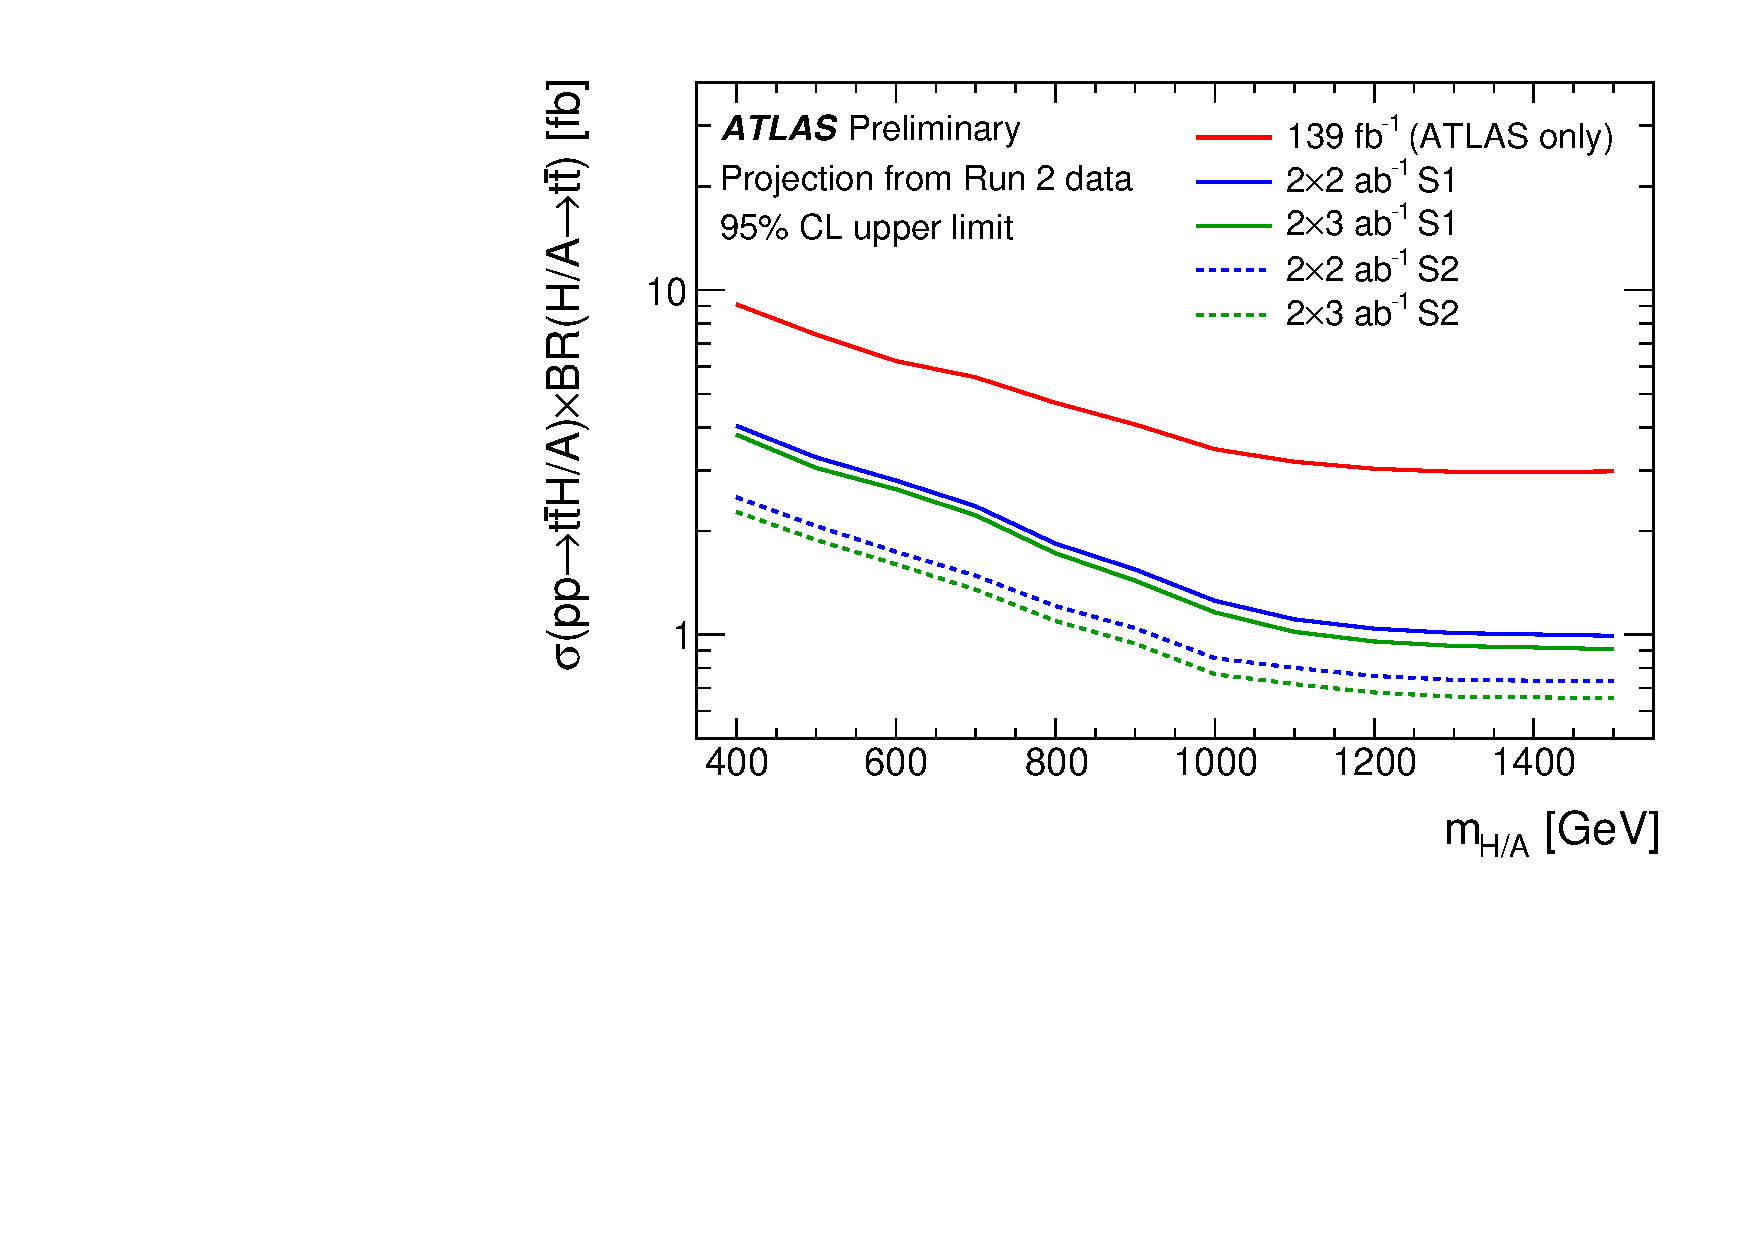
\includegraphics[width=0.75\textwidth]{figures/Projection/HA_tttt.pdf}
\caption{Projected 95\% CL upper limits on $\boldsymbol{\sigma(pp \to t\bar{t}H/A)\times\mathcal{B}(H/A \to t\bar{t})}$ as a function of $\boldsymbol{m_{H/A}}$ for different integrated luminosities and systematic uncertainty scenarios.}
\label{fig:HL_HA_limits}
\end{figure}

The interplay between systematic and statistical effects is further illustrated by the luminosity evolution shown in Figure~\ref{fig:HL_HA_lumi} for representative resonance masses of 400~GeV and 1.5~TeV. 
For the 400~GeV benchmark, the improvement saturates beyond approximately 1~ab$^{-1}$, indicating that systematic uncertainties dominate the sensitivity. 
Conversely, for the 1.5~TeV benchmark, the limits continue to improve steadily with increasing luminosity, reflecting the limited signal yield in this mass regime. 
This behaviour underscores the complementary roles of increased dataset size and improved theoretical modelling in fully exploiting the HL-LHC potential.

\begin{figure}[htbp]
\centering
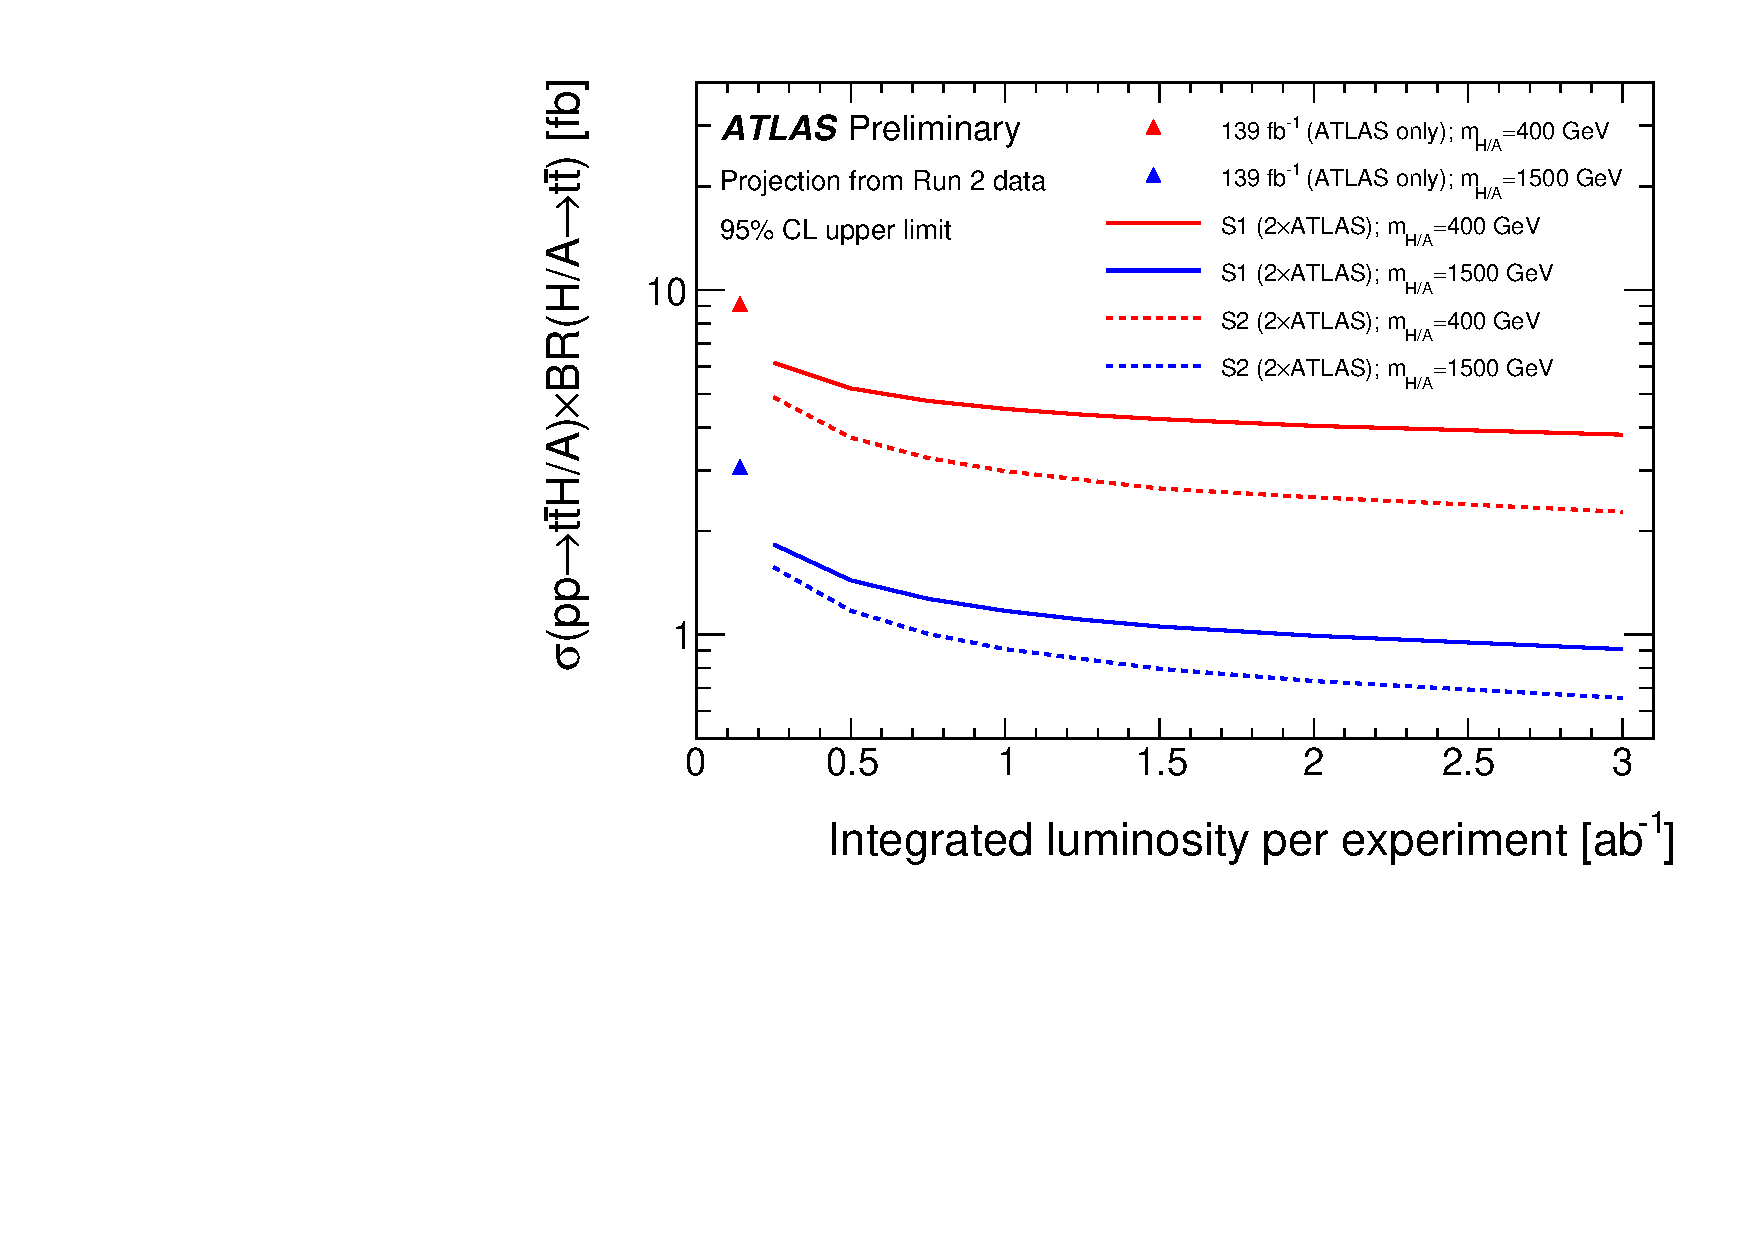
\includegraphics[width=0.75\textwidth]{figures/Projection/HA_lumi.pdf}
\caption{Projected 95\% CL upper limits on $\boldsymbol{\sigma(pp \to t\bar{t}H/A)\times\mathcal{B}(H/A \to t\bar{t})}$ as a function of integrated luminosity for representative resonance masses.}
\label{fig:HL_HA_lumi}
\end{figure}

To quantify the discovery reach, benchmark $H/A$ signals are injected with cross-sections of 6.1, 3.3 and 2.0~fb for resonance masses of 400, 800 and 1500~GeV, respectively. 
These values correspond to an expected local significance of approximately three standard deviations with 1~ab$^{-1}$ per experiment under Scenario~2.

With increasing luminosity, the projected significances approach or exceed the five-standard-deviation threshold, reaching 5.2, 5.4 and 5.5 standard deviations for 3~ab$^{-1}$ per experiment. 
This demonstrates that the HL-LHC will not only strengthen exclusion limits but also provide genuine discovery potential for heavy $H/A$ resonances close to the current sensitivity frontier.

\subsubsection{Top-Philic Scalar Resonances ($S_8$ and $S_1$)}
\label{sec:HL_top_philic}

The projected 95\% CL upper limits on 
$\sigma(pp \to S_8 S_8)\times \mathcal{B}(S_8 \to t\bar{t})^2$ 
are shown in Figure~\ref{fig:HL_S8_limits}. 
The particularly strong sensitivity to $S_8$ arises from its QCD-driven pair-production mechanism, which yields comparatively large cross-sections even at TeV-scale masses.

The most stringent expected limit is obtained around $m_{S_8}\sim1.2$~TeV, reaching approximately 0.3~fb in the combined ATLAS and CMS projection under Scenario~2. 
For masses above 1~TeV, the projected limits remain below 1~fb over a broad mass range.

\begin{figure}[htbp]
\centering
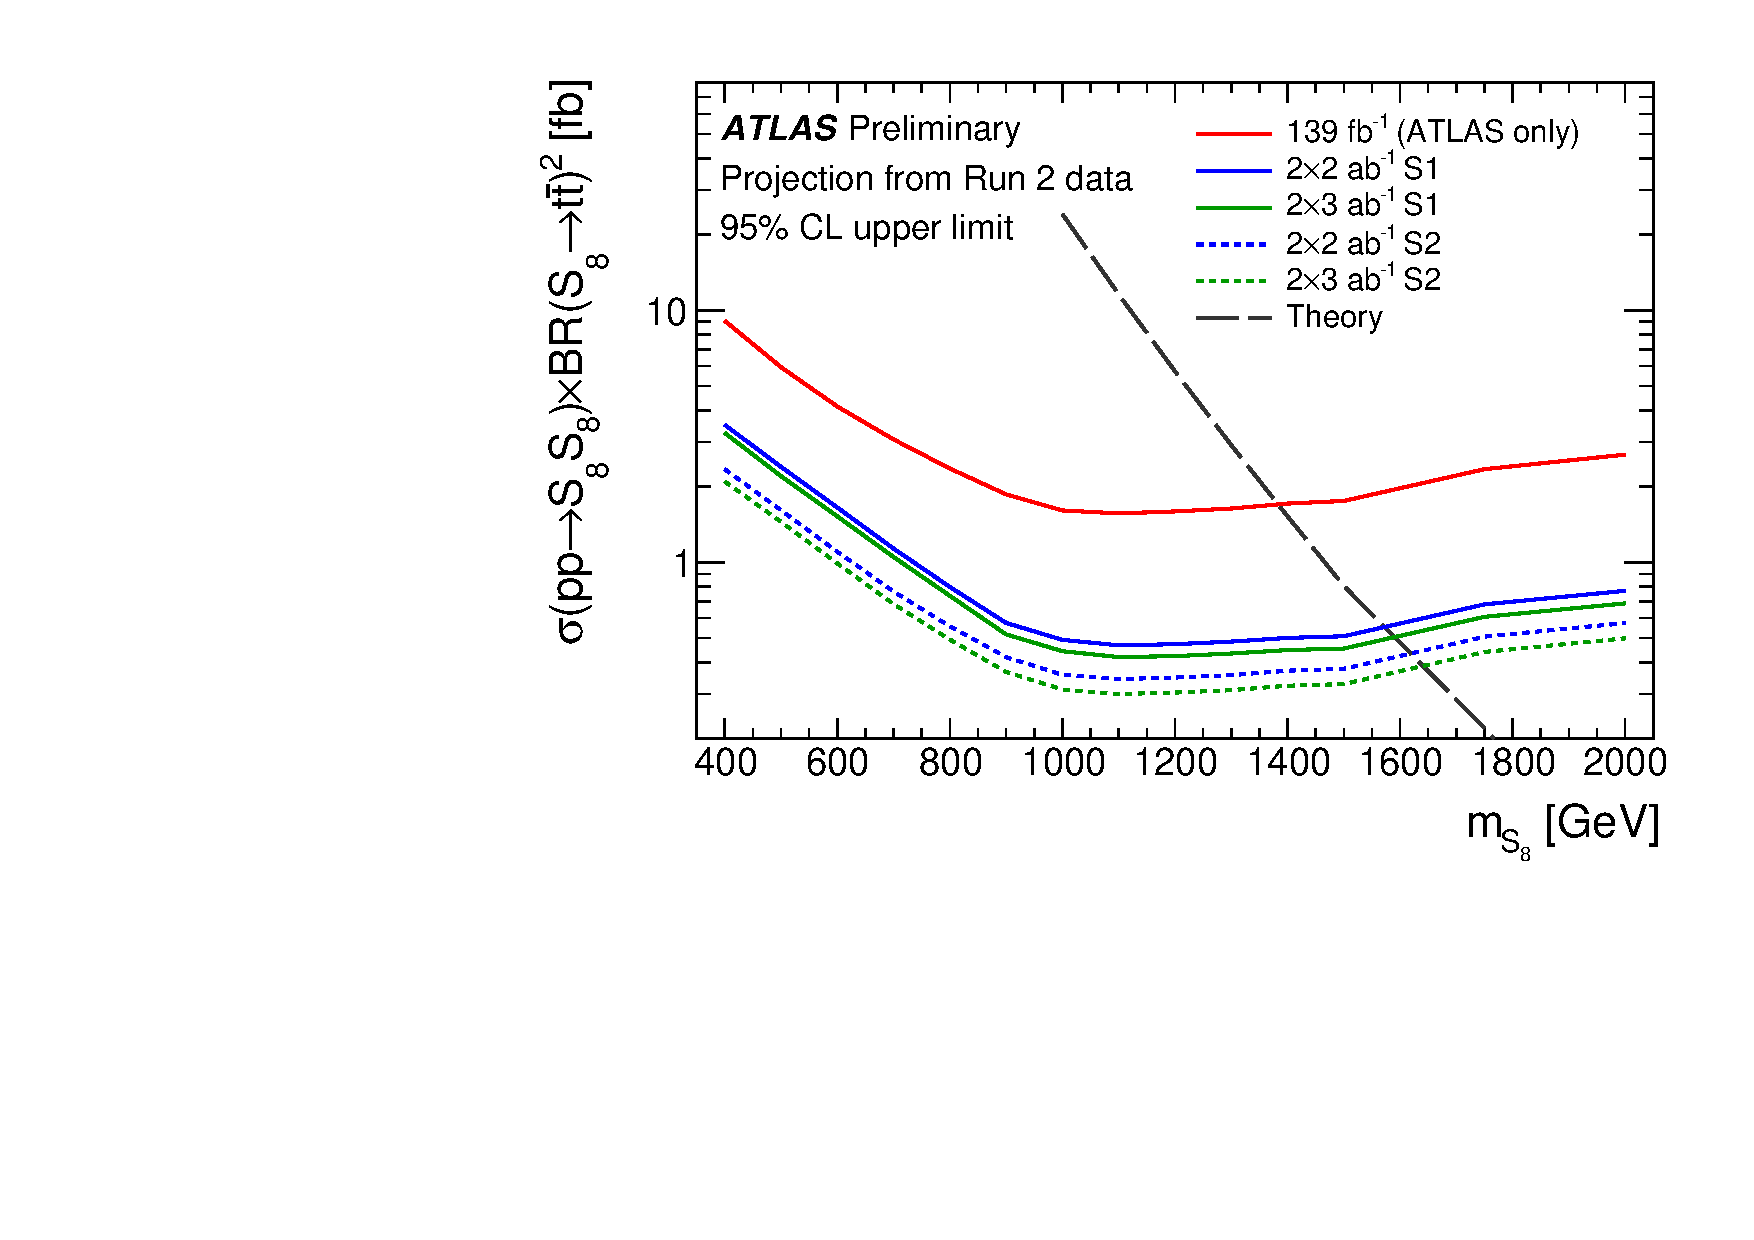
\includegraphics[width=0.75\textwidth]{figures/Projection/S8_tttt.pdf}
\caption{Projected 95\% CL upper limits on $\boldsymbol{\sigma(pp \to S_8 S_8)\times \mathcal{B}(S_8 \to t\bar{t})^2}$ as a function of $\boldsymbol{m_{S_8}}$.}
\label{fig:HL_S8_limits}
\end{figure}

For the colour-singlet scalar $S_1$, the projected cross-section limits depend on both the mass and the coupling to top quarks, $y_{S_1}$, reflecting modifications of both the production rate and the resonance width.

The projected upper limits on 
$\sigma(pp \to t\bar{t}S_1)\times \mathcal{B}(S_1 \to t\bar{t})$ 
for two representative coupling choices are shown in Figure~\ref{fig:HL_S1_mass}. 
Figure~\ref{fig:HL_S1_mass}(a) corresponds to $y_{S_1}=0.1$, while Figure~\ref{fig:HL_S1_mass}(b) corresponds to $y_{S_1}=2.0$. 
The mild irregularities observed in the limits arise from the finite size of the simulated samples.

\begin{figure}[htbp]
\centering

\begin{subfigure}[t]{0.48\textwidth}
    \centering
    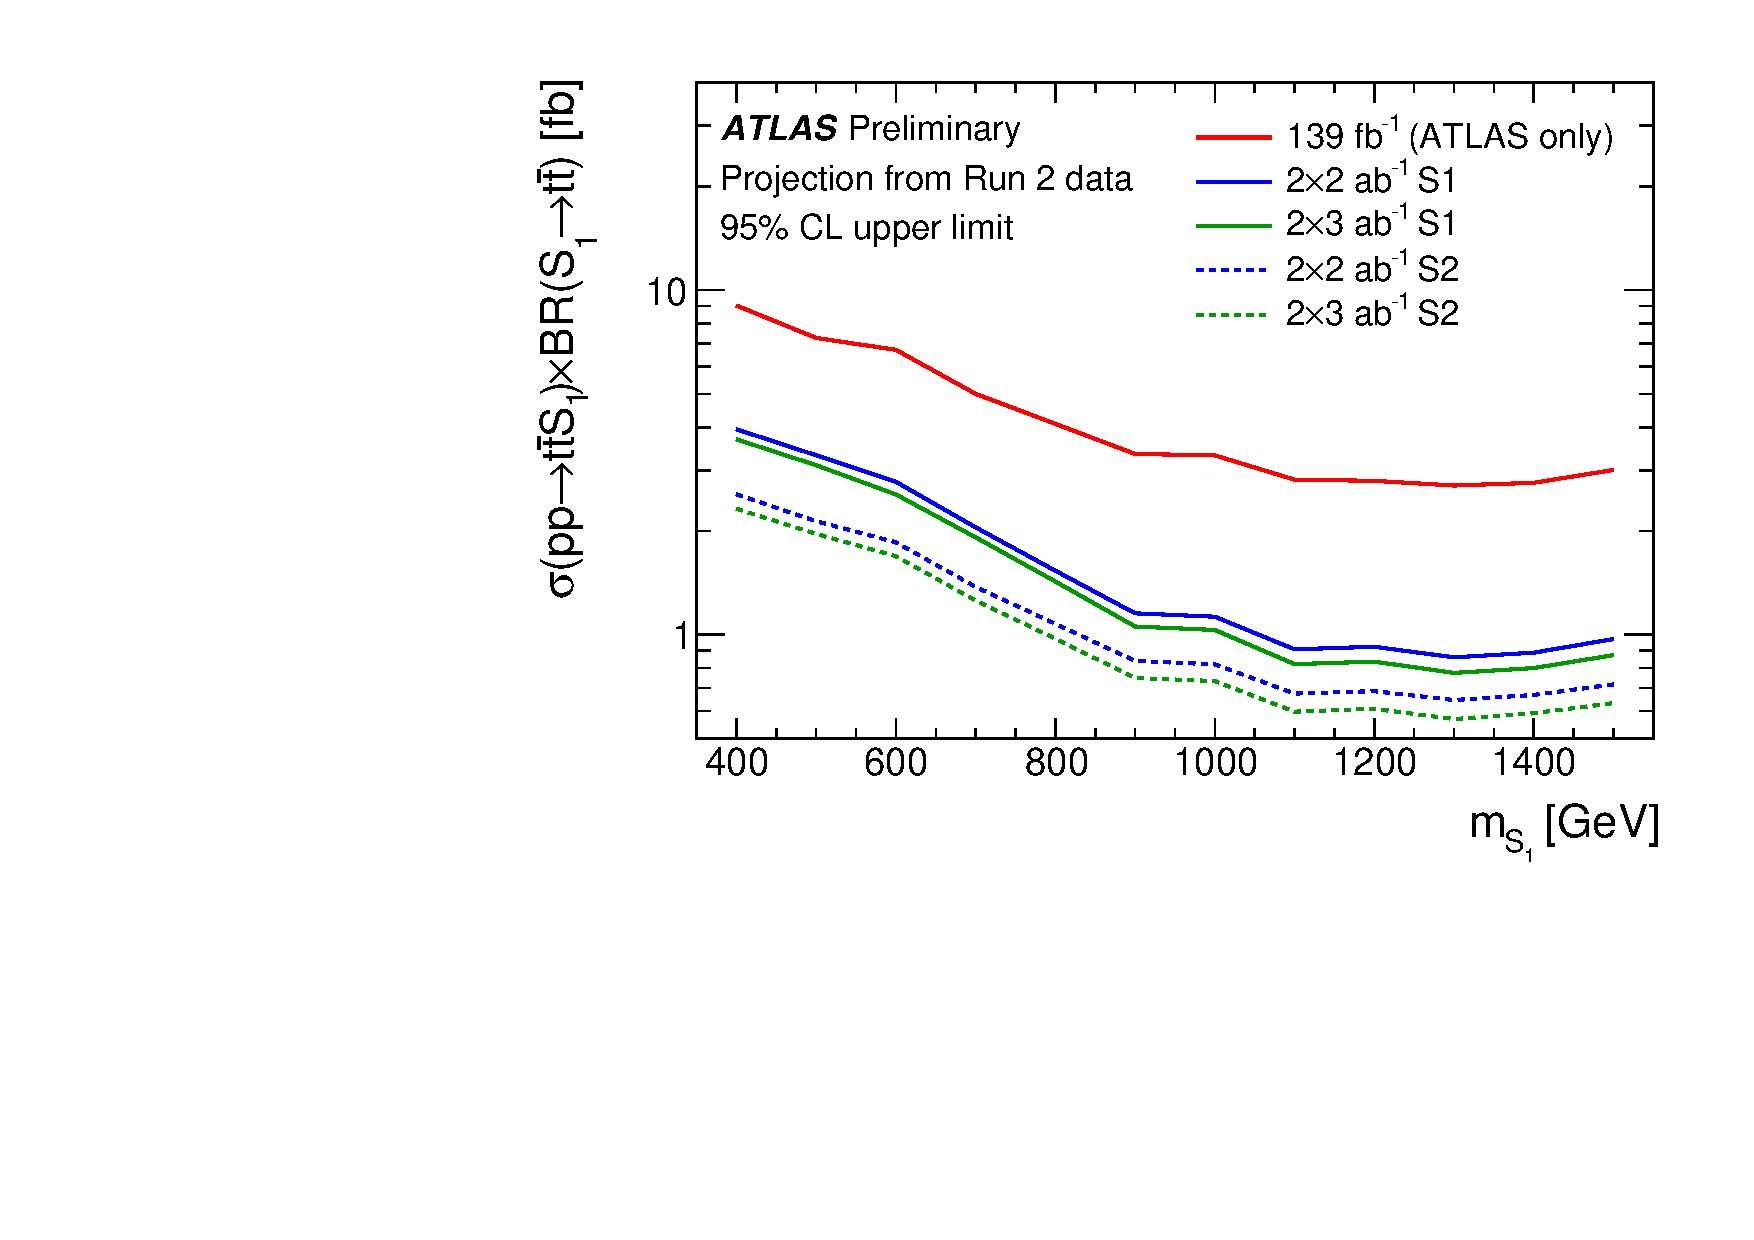
\includegraphics[width=\textwidth]{figures/Projection/S1_tttt_y0p1.pdf}
    \caption{$\boldsymbol{y_{S_1}=0.1}$}
\end{subfigure}
\hfill
\begin{subfigure}[t]{0.48\textwidth}
    \centering
    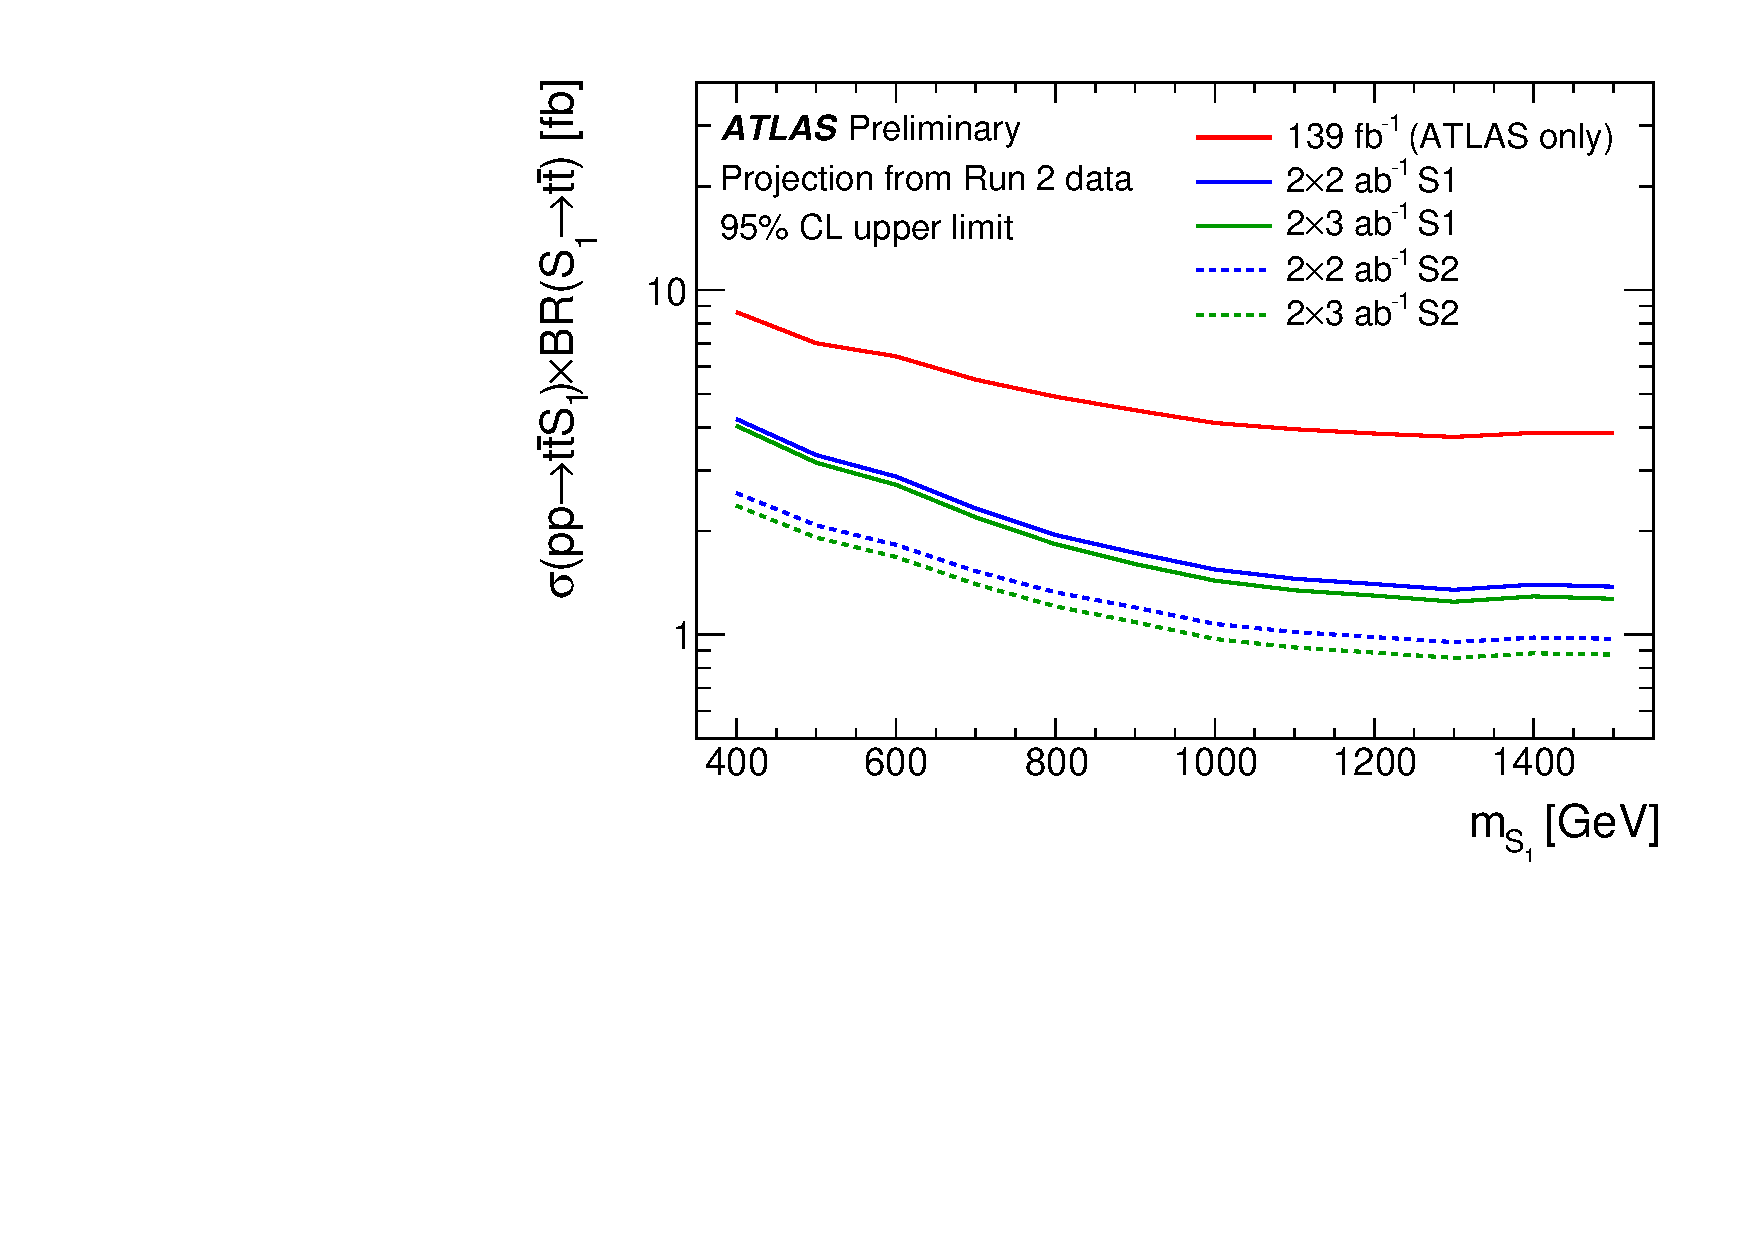
\includegraphics[width=\textwidth]{figures/Projection/S1_tttt_y2p0.pdf}
    \caption{$\boldsymbol{y_{S_1}=2.0}$}
\end{subfigure}

\caption{Projected 95\% CL upper limits on 
$\boldsymbol{\sigma(pp \to t\bar{t}S_1)\times \mathcal{B}(S_1 \to t\bar{t})}$ 
as a function of $\boldsymbol{m_{S_1}}$ for two representative coupling values.}
\label{fig:HL_S1_mass}
\end{figure}

To derive exclusion contours in the parameter space, the projected cross-section limits are compared to the theoretical predictions, resulting in the exclusion regions shown in Figure~\ref{fig:HL_S1_plane}.
At $m_{S_1}=400$~GeV, values of $y_{S_1}$ above approximately 0.17 are excluded with 3~ab$^{-1}$ per experiment under Scenario~2. 
At $m_{S_1}=1.5$~TeV, couplings above roughly 0.8--0.95 are excluded depending on the luminosity and systematic scenario.

\begin{figure}[htbp]
\centering
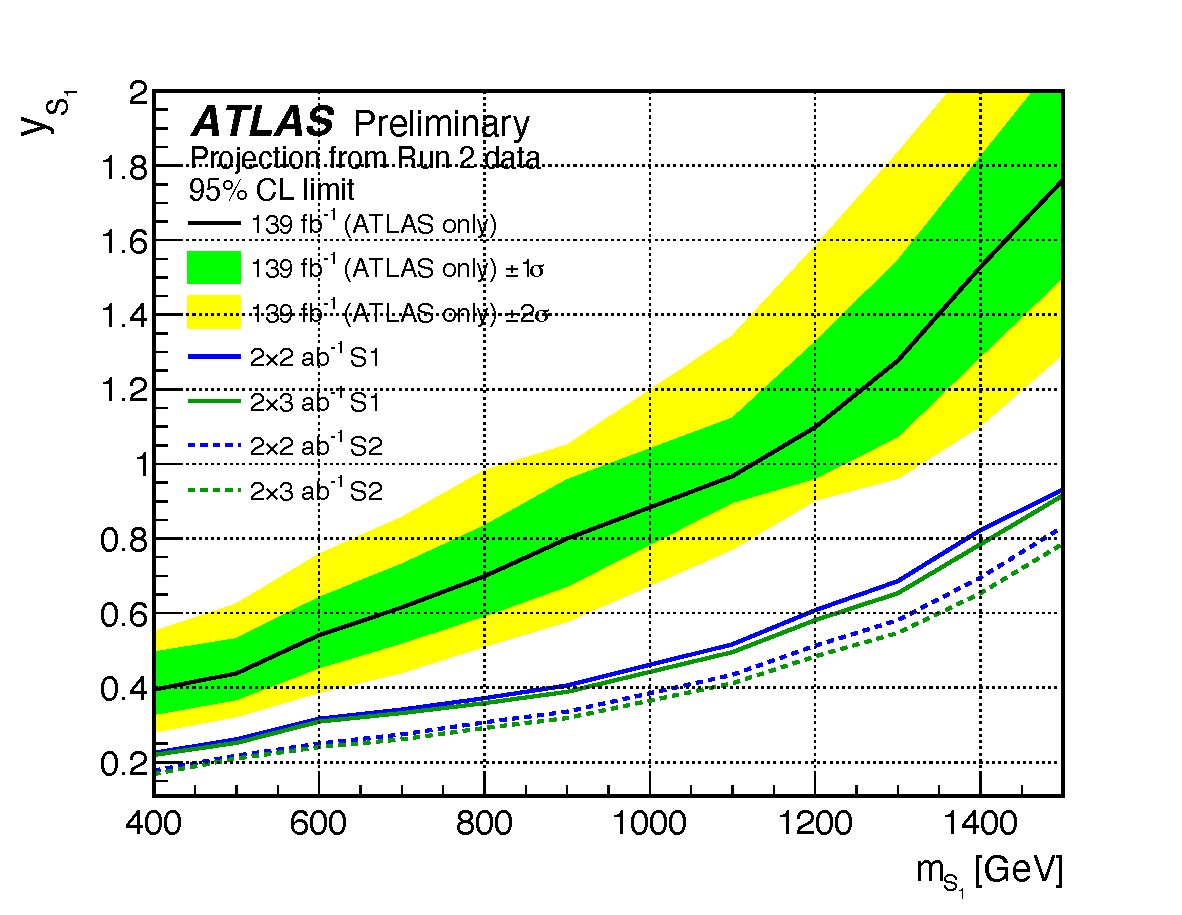
\includegraphics[width=0.75\textwidth]{figures/Projection/S1_2D.pdf}
\caption{Projected 95\% CL exclusion contours in the $\boldsymbol{(m_{S_1}, y_{S_1})}$ plane under different luminosity and systematic assumptions.}
\label{fig:HL_S1_plane}
\end{figure}